\documentclass[oneside]{book}

\setcounter{tocdepth}{1}
\setcounter{secnumdepth}{3}

\usepackage[toc,page]{appendix}
\usepackage{hyperref}
\usepackage[utf8]{inputenc}
\usepackage{graphicx} % Required for the inclusion of images
\usepackage{amsmath} % Required for some math elements 
\usepackage[utf8]{inputenc}
\usepackage[english]{babel}
\newtheorem{theorem}{Theorem}
\newtheorem{corollary}{Corollary}[theorem]
\newtheorem{lemma}[theorem]{Lemma}
\usepackage{listings}
\usepackage{pdfpages}
\usepackage{amssymb}
\usepackage{pdflscape}

\begin{document}

\begin{titlepage}
	\centering
	
\includegraphics[width=0.60\textwidth]{../../logo/UoN_Primary_Logo_RGB.png}\par\vspace{1cm}
	\vspace{1.5cm}
	{\huge\bfseries Comparing the Pure Functional and Object Oriented Paradigm for implementing ABS \par}
	\vspace{2cm}
	{\Large\itshape jonathan.thaler@nottingham.ac.uk \par}
	\vfill
	
	\vfill

	{\large \today\par}
\end{titlepage}

\cleardoublepage

\section*{Abstract}
This study we compares the object oriented and pure functional programming paradigms to implement Agent-Based Simulation. Due to fundamentally different concepts both propagate fundamental different approaches in implementing ABS. In this document we seek to precicesly identify these fundamental differences, compare them and also look into general benefits and drawbacks of each approach.

\clearpage
\tableofcontents
\clearpage

\section{Introduction}
There exists a large number of simulation packages which allow the convenient creation of System Dynamics simulations by straight-forward visual diagram creation. One simply creates stocks and flows, connects them, specifies the flow-rates and initial parameters and then runs the model. An example for such a visual diagram creation in the simulation package AnyLogic can be seen in Figure \ref{fig:sir_stockflow_diagram}.

\begin{figure}
	\centering
	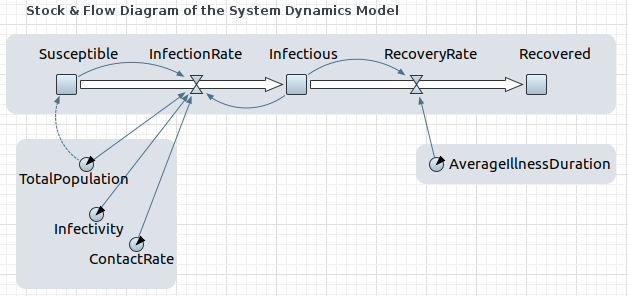
\includegraphics[width=.5\textwidth, angle=0]{./fig/SIR_SD_STOCKFLOW_DIAGRAMM.png}
	\caption{Visual System Dynamics Diagram of the SIR model in AnyLogic Personal Learning Edition 8.3.1.}
	\label{fig:sir_stockflow_diagram}
\end{figure}

Still, implementing System Dynamics directly in code is not as straight forward and involves numerical integration which can be quite tricky to get right. Thus, the aim of this paper is to look into how System Dynamics models can be implemented in code correctly without the use of a simulation package. We use the well known SIR model \cite{kermack_contribution_1927} from epidemiology to demonstrate our approach.

Our language of choice is Haskell because it emphasises a declarative programming style in which one describes \textit{what} instead of \textit{how} to compute. Further it allows to rule out interference with non-deterministic influences or side-effects already at compile-time. This is of fundamental importance for System Dynamics because it behaves completely deterministic and involves no stochastics or non-determinism whatsoever. Also, we make use of Functional Reactive Programming which allows to express continuous-time systems in a functional way. 

We show that by this approach we can arrive at correct-by-construction implementations of System Dynamic models. This means that the correctness of the code is obvious because we have closed the gap between the model specification and its implementation. Thus, the contribution of the paper is the demonstration of how to implement correct-by-construction System Dynamics simulations using Haskell and Functional Reactive Programming.

\section{Programming paradigms and ABS}
In this section we give a brief overview of comparing the suitability of three fundamentally different languages to implement the different update-strategies. We wanted to cover a wide range of different types of languages and putting emphasis on each languages strengths without abusing language constructs to recreate features it might seem to lack. An example would be to rebuild OO constructs in pure functional languages which would be a abuse of the language, something we explicitly avoided although it resulted in a few limitations as noted below. We implemented both the \textit{Prisoners Dilemma} game on a 2D grid and the \textit{Heroes \& Cowards} game in all three languages with all four update-strategies. \footnote{Code available under\\ \url{https://github.com/thalerjonathan/phd/tree/master/coding/papers/iteratingABM/}}
TODO: reference table:

\subsection{OO: Java}
This language is included as the benchmark of object-oriented (OO) imperative languages as it is extremely popular in the ABS community and widely used in implementing their models and frameworks. It comes with a comprehensive programming library and powerful synchronization primitives built in at language-level.

\paragraph{Ease of Use}
We found that implementing all the strategies was straight-forward and easy thanks to the languages features. Especially parallelism and concurrency is convenient to implement due to elegant and powerful built-in synchronization primitives.

\paragraph{Benefits}
We experienced quite high-performance even for a large number of agents which we attributed to the implicit side-effects using aliasing through references. This prevents massive copying like Haskell but comes at the cost of explicit data-flow.

\paragraph{Deficits}
A downside is that one must take care when accessing memory in case of \textit{parallel} or \textit{concurrent strategy}. Due to the availability of aliasing and side-effects in the language it can't be guaranteed by Java's type-system that access to memory happens only when its safe. So care must be taken when accessing references sent by messages to other agents, accessing references to other agents or the infrastructure of an agent itself e.g. the message-box. We found that implementing the \textit{actor strategy} was not possible when using thousands of agents because Java can't handle this number of threads. For implementing the \textit{parallel} and \textit{concurrent} ones we utilized the ExecutorService to submit a task for each agent which runs the update and finishes then. The tasks are evenly distributed between the available threads using this service where the service is backed by the number of cores the CPU has. This approach does not work for the \textit{actor strategy} because there an agent runs constantly within its thread making it not possible to map to the concept of a task as this task would not terminate. The ExecutorService would then start n tasks (where n is the number of threads in the pool) and would not start new ones until those have finished, which will not occur until the agent would shut itself down. Also yielding or sleeping does not help either as not all threads are started but only n. 

\paragraph{Natural Strategy}
We found that the \textit{sequential strategy} with immediate message-handling is the most natural strategy to express in Java due to its heavy reliance on side-effects through references (aliases) and shared thread of execution. Also most of the models work this way making Java a save choice for implementing ABS.





 
\subsection{Pure functional: Haskell}
This language is included to put to test whether a pure functional, declarative programming language is suitable for full-blown ABS. What distinguishes it is its complete lack of implicit side-effects, global data, mutable variables and objects. The central concept is the function into which all data has to be passed in and out explicitly through statically typed arguments and return values: data-flow is completely explicit. For a nice overview on the features and strengths of pure functional programming see the classical paper  \cite{hughes_why_1989}.

\paragraph{Ease of Use}
We initially thought that it would be suitable best for implementing the \textit{parallel strategy} only due the inherent data-parallel nature of pure functional languages. After having implementing all strategies we had to admit that Haskell is very well suited to implement all of them faithfully. We think this stems from the fact that it has no implicit side-effects which reduces bugs considerably and results in completely explicit data-flow. 
Not having objects with data and methods, which can call between each other meant that we needed some different way of representing agents. This was done using a struct-like type to carry data and a transformer function which would receive and process messages. This may seem to look like OO but it is not: agents are not carried around but messages are sent to a receiver identified by an id.

\paragraph{Benefits}
Haskell has a very powerful static type-system which seems to be restrictive in the beginning but when one gets used to it and knows how to use it for ones support, then it becomes rewarding. Our major point was to let the type-system prevent us from introducing side-effects. In Haskell this is only possible in code marked in its types as producing side-effects, so this was something we explicitly avoided and were able to do so throughout the whole implementation. This means a user of this approach can be guided by the types and is prevented from abusing them. In essence, the lesson learned here is \textit{if one tries to abuse the types or work around, then this is an indication that the update-strategy one has selected does not match the semantics of the model one wants to implement}. If this happens in Java, it is much more easier to work around by introducing global variables or side-effects but this is not possible in Haskell. Also we claim that when using Haskell one arrives at a much safer version in the case of Parallel or Concurrent Strategies than in Java.

Parallelism and Concurrency is extremely convenient to implement in Haskell due to its complete lack of implicit side-effects. Adding hardware-parallel execution in the \textit{parallel strategy} required the adoption of only 5 lines of code and no change to the existing agent-code at all (e.g. no synchronization, as there are no implicit side-effects). For implementing the \textit{concurrent strategy} we utilized the programming model of Software-Transactional-Memory (STM). The approach is that one optimistically runs agents which introduce explicit side-effects in parallel where each agent executes in a transaction and then to simply retry the transaction if another agent has made concurrent side-effect modifications. This frees one from thinking in terms of synchronization and leaves the code of the agent nearly the same as in the \textit{sequential strategy}. 
Spawning thousands of threads in the \textit{actor strategy} is no problem in Haskell due to its lightweight handling of threads internal in the runt-time system, something which Java seems to be lacking. We have to note that each agents needs to explicitly yield the execution to allow other agent-threads to be scheduled, something when omitted will bring the system to a grind.

\paragraph{Deficits}
Performance is an issue. Our Haskell solution could run only about 2000 agents in real-time with 25 updates per second as opposed to 50.000 in our Java solution, which is not very fast. It is important though to note, that being beginners in Haskell, we are largely unaware of the subtle performance-details of the language so we expect to achieve a massive speed-up in the hands of an experienced programmer.

Another thing is that currently only homogeneous agents are possible and still much work needs do be done to capture large and complex models with heterogeneous agents. For this we need a more robust and comprehensive surrounding framework, which is already existent in the form of functional reactive programming (FRP). Our next paper is targeted on combining our Haskell solution with an FRP framework like Yampa (see Further Research). 

Our solution so far is unable to implement the \textit{sequential strategy} with immediate message-handling. This is where OO really shines and pure functional programming seems to be lacking in convenience. A solution would need to drag the collection of all agents around which would make state-handling and manipulation very cumbersome. In the end it would have meant to rebuild OO concepts in a pure functional language, something we didn't wanted to do. For now this is left as an open, unsolved issue and we hope that it could be solved in our approach with FRP (see future research).

\paragraph{Natural Strategy}
The most natural strategy is the \textit{parallel strategy} as it lends itself so well to the concepts of pure functional programming where things are evaluated virtually in parallel without side-effects on each other - something which resembles exactly the semantics of the \textit{parallel strategy}. We argue that with slightly more effort, the \textit{concurrent strategy} is also very natural formulated in Haskell due to the availability of STM, something only possible in a language without implicit side-effects as otherwise retries of transactions would not be possible.



\subsection{Multi-paradigm: Scala}
%TODO: implement other strategies
%TODO: much shorter than the other two, because not implemented all and not so much to say

This multi-paradigm functional language which sits in-between Java and Haskell and is included to test the usefulness of the \textit{actor strategy} for implementing ABS. The language comes with an Actor-library inspired by \cite{agha_actors:_1986} and resembles the approach of Erlang which allows a very natural implementation of the strategy.

\paragraph{Ease of Use}
We were completely new to Scala with Actors although we have some experience using Erlang which was of great use. We found that the language has some very powerful mixed-paradigm features which allow to program in a very flexible way without inducing too much restrictions on one.

\paragraph{Benefits}
Implementing agent-behaviour is extremely convenient, especially for simple state-driven agents. The Actor-language has a built-in feature which allows to change the behaviour of an agent on message-reception where the agent then simply switches to a different message-handler, allowing elegant implementation of state-dependent behaviour. 

Performance is very high. We could run simulations in real-time with about 200.000 agents concurrently, thanks to the transparent handling in the run-time system. Also it is very important to note that one can use the framework Akka to build real distributed systems using Scala with Actors so there are potentially no limits to the size and complexity of the models and number of agents one wants to run with it.

\paragraph{Deficits}
Care must be taken not to send references and mutable data, which is still possible in this mixed-paradigm language.

\paragraph{Natural Strategy}
The most natural strategy would be of course the \textit{actor strategy} and we only used this strategy in this language to implement our models. Note that the \textit{actor strategy} is the most general one and would allow to capture all the other strategies using the appropriate synchronization mechanisms.



\begin{table*}[t]
\centering
\caption{Language Comparisons}
\label{tab:language_comparisons}
\begin{tabular}{l || l | l | l  }
	 			& Java 	& Haskell 	& Scala	\\ \hline \hline

Sequential		& ++	& --		& ? (+)		\\  
Parallel		& +		& ++		& ?	(+)	\\  
Concurrent		& +		& +			& ?	(+)	\\  
Actor			& --	& +			& ++	\\  

\end{tabular}
\end{table*}

\renewcommand\bibname{References}

\bibliographystyle{acm}
\bibliography{../../references/phdReferences}

\end{document}
